\section{Fase di lookup}
\subsection{Introduzione}
Una volta terminata la fase di Boot, il peer può iniziare a inoltrare al proprio superpeer richieste di ricerca. La fase di lookup (ricerca) riveste un ruolo fondamentale nell' applicazione, in quanto l'abilità di trovare almeno un istanza di un oggetto è molto importante, altrimenti non sarebbe possibile procedere alla successiva fase di download del file da uno dei peer ottenuti come risposta da questa fase.\linebreak

\subsection{Ricerca}
La ricerca da parte di altri peer possessori di un determinato file è svolta in maniera indiretta dal peer, in quanto il lavoro piu grande viene svolto dal suo superpeer. \linebreak
Le ricerche sono effettuate in maniera sequenziale, durante questa fase le operazioni che il peer può effettuare sono solamente l'update, lo stop della ricerca e l'invio del ping al proprio superpeer. Non è possibile effettuare ricerche in parallelo.\linebreak
Per lo scambio di messaggi nella fase di lookup è stato creato un pacchetto specifico (pacchetto whohas), con la seguente struttura:\linebreak

\begin{figure}[h]
\centering
{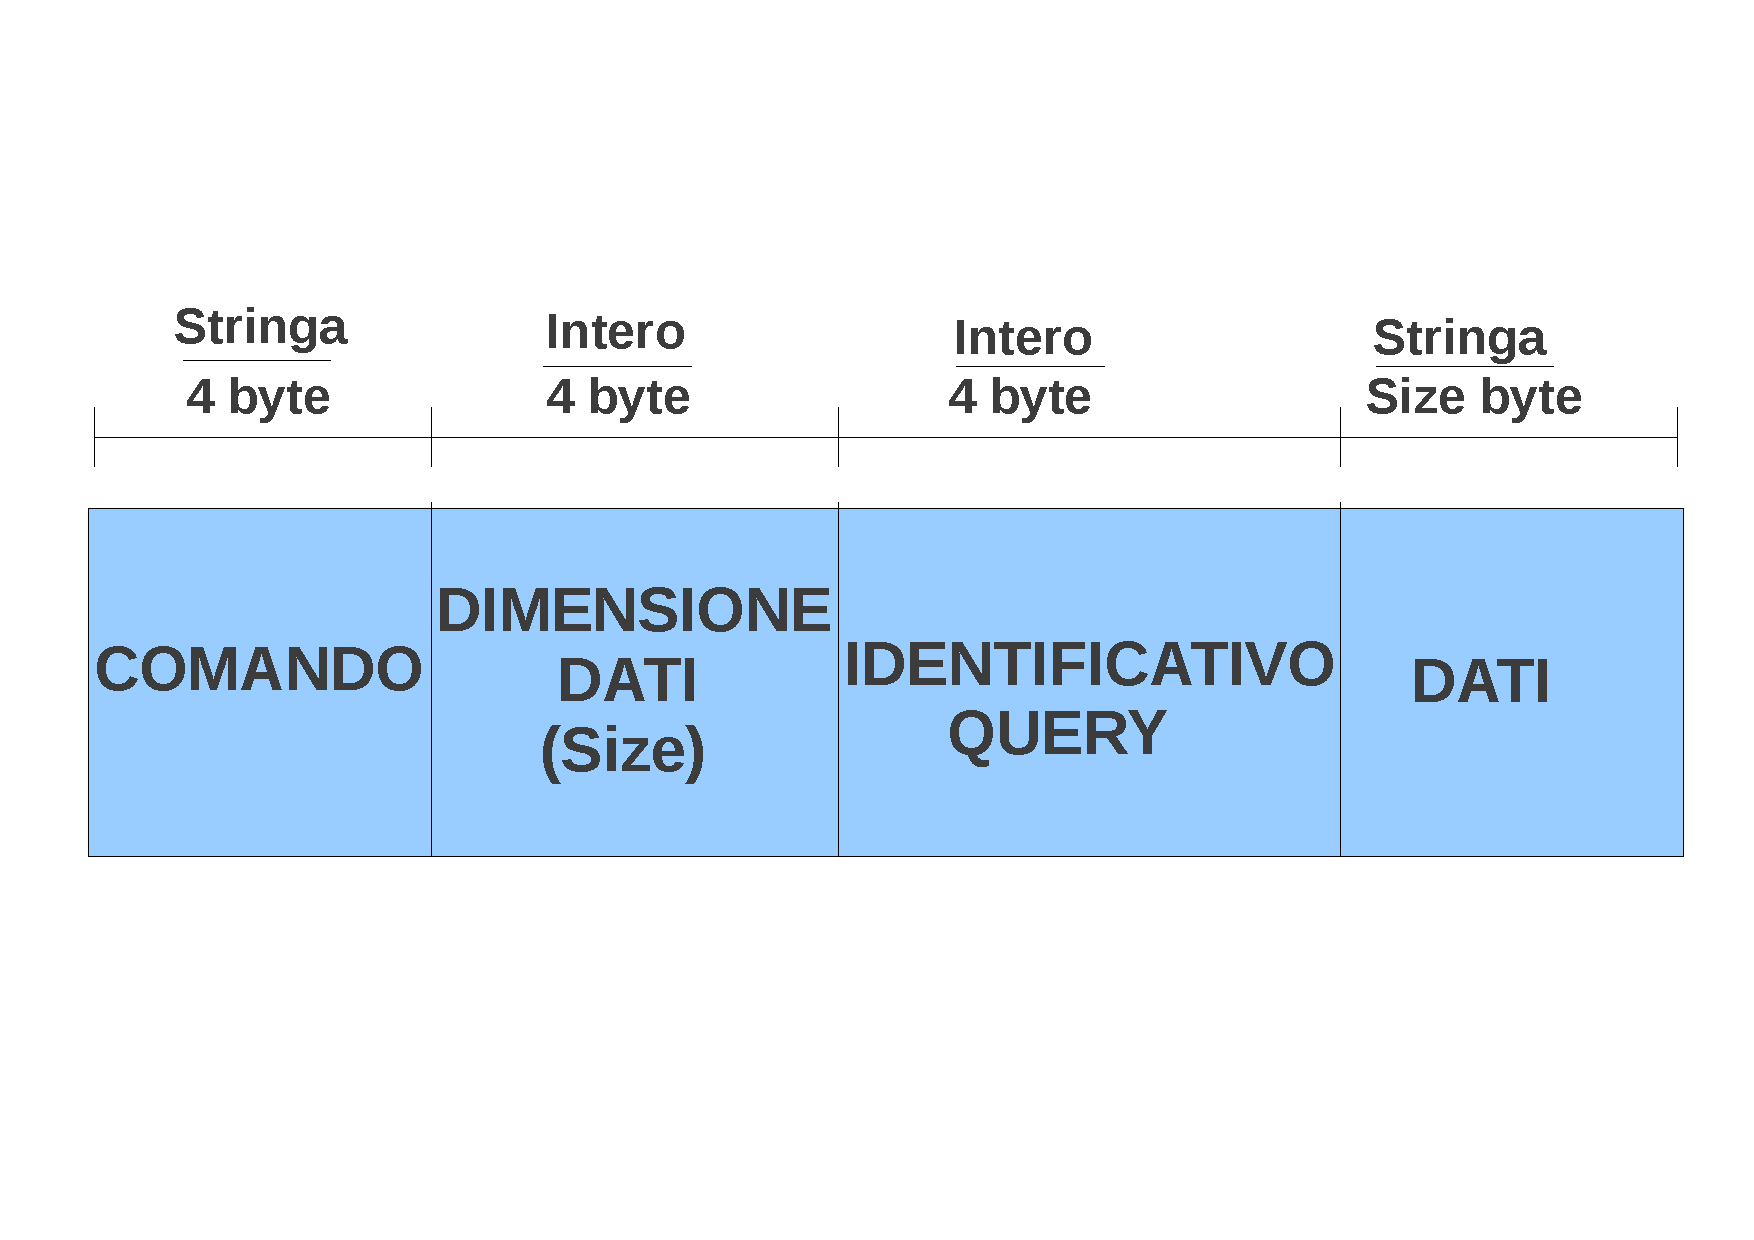
\includegraphics[width=10cm]{img/pck_whhs}}
\caption{struttura pacchetto per la whohas}
\end{figure}

La fase di lookup può essere suddivisa in 3 sottofasi principali:\linebreak
\begin{itemize}
\item Invio richiesta di ricerca da parte del peer al proprio superpeer, e attesa delle relative risposte;
\item Ricerca da parte del superpeer dei peer a lui collegati che possiedono il file richiesto, inoltro della richiesta sull'overlay e attesa risposte dall'overlay, gestione risposte ricevute e inoltro dei risultati al peer che stà effettuando la ricerca;
\item Fine della ricerca; in seguito, il peer che ha effettuato la ricerca, se ci sono dei peer che possiedono il file, effettuerà il download del file cercato da uno dei peer restituiti.
\end{itemize}

\subsubsection{Richiesta da parte del peer al superpeer}
Quando un utente decide di avviare una ricerca dovrà selezionare nel menù il comando di whohas. Inserito il comando da terminale, verrà richiesto il nome del file da cercare (il nome non può essere abbreviato ma deve essere esattamente uguale al nome completo del file, eccezione fatta per le maiuscole e le minuscole). Una volta inserite queste informazioni l'applicazione provvederà a creare il pacchetto di tipo whohas descritto precedentemente, con i relativi campi riempiti come segue:\linebreak
\begin{itemize}
\item Comando = "whhs";
\item Size = dimensione in byte del nome del file da cercare;
\item Identificativo whohas (ID) = 0;
\item Dati = nome del file da cercare.
\end{itemize}
Una volta creato il pacchetto, questo verrà passato alla socket UDP che provvederà a inoltrarlo verso il superpeer di destinazione. Si noti come un pacchetto whohas inviato da un peer verso il proprio superpeer abbia sempre identificativo uguale a 0 (questo per permettere al superpeer di distinguere le whohas ricevute dai propri peer da quelle ricevute dagli altri superpeer nella rete di overlay, le quali hanno sempre identificativo diverso da zero, come vedremo successivamente). Si conclude questa parte illustrando lo scambio di messaggi tra peer e superpeer associato durante una ricerca, trascurando momentaneamente il dettaglio su come poi il superpeer interagisca con gli altri superpeer della rete di overlay e la fine della ricerca.

\begin{figure}[h]
\centering
{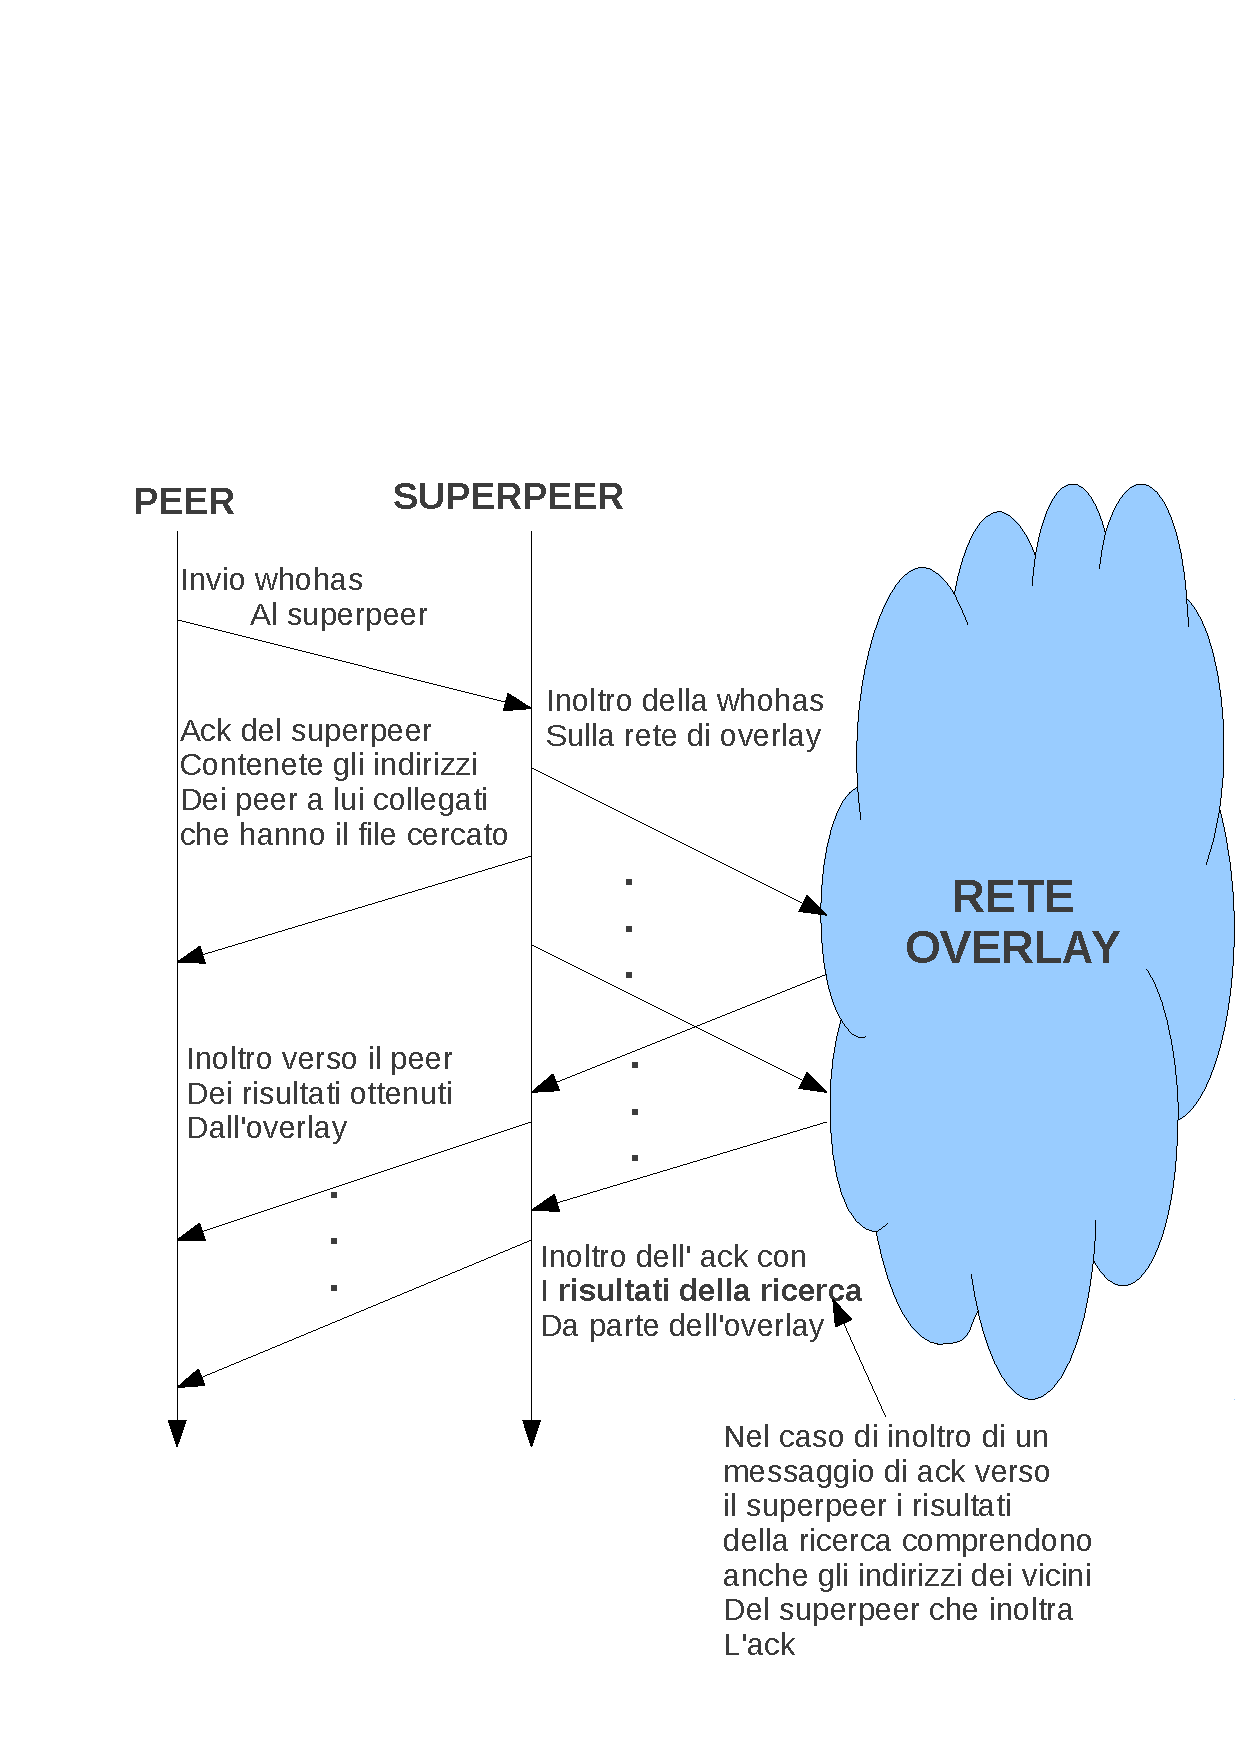
\includegraphics[width=9cm]{img/scambio_msg_whhs}}
\caption{Scambio di messaggi tra peer e superpeer durante una ricerca}
\end{figure}
 
  
\subsubsection{Ricerca dei peer possessori del file da parte del superpeer}
Quando un superpeer riceve sulla sua socket UDP un messaggio di whohas, si crea il pacchetto dal buffer della socket attraverso apposite funzioni di parsing e memorizzazione. Se il comando ricevuto è uguale a "whhs" e la richiesta è stata inoltrata da un peer che è collegato a questo superpeer, come prima cosa il superpeer controlla il valore del campo ID: se quest'ultimo è pari a zero, si entrerà nella parte di codice relativa alla gestione della whohas ricevuta da un propio peer (nuova ricerca).\linebreak
Anche se la ricerca a livello di peer è sequenziale, il superpeer deve poter gestire più ricerche attive in parallelo e nasce quindi l'esigenza di distinguere le varie ricerche pendenti. Per far ciò, quando il superpeer riceve una whohas con identificativo pari a 0, assegna alla query corrispondente un nuovo ID univoco (a livello locale di superpeer), assegnato in maniera incrementale. \linebreak
Una volta assegnato un nuovo ID alla whohas (di una nuova ricerca), il superpeer ricava il nome del file di cui si vogliono conoscere i possessori dal campo dati del pacchetto e inoltre memorizza anche l'indirizzo IP del peer che ha inviato la richiesta. Per la gestione di query pendenti, il superpeer utilizza una lista (lista\_query) che contiene le seguenti informazioni:\linebreak

\begin{itemize}
\item ID della query (assegnata dal superpeer);
\item IP del peer che ha inoltrato la query;
\item Nome del file da cercare;
\item Un contatore per mantenere l'informazione su quanti superpeer sono già stati contattati;
\item Un contatore per mantenere l'informazione su quanti IP di peer si sono già ricevuti in risposta;
\item Due liste di indirizzi IP (try\_list, done\_list, il cui scopo verrà illustrato in seguito).
\end{itemize}
  
Dopo aver effettuato i controlli descritti precedentemente ed aver inserito la query appena ricevuta nella lista delle query pendenti, il superpeer come prima cosa verifica se tra i suoi peer c'è qualcuno che possiede il file richiesto. In caso affermativo inoltra un pacchetto whohas il cui comando viene settato ad "ack", ID a zero, il campo dati con gli indirizzi IP dei peer che possiedono il file e il campo size con il numero di byte presenti nel campo dati, inoltre viene aggiornato anche il contatore in lista\_query relativo al numero di IP di peer che hanno il file cercato. Nel caso in cui nessuno dei suoi peer abbia il file cercato invierà un pacchetto whohas con comando settato ad "ack", ID a zero, campo dati vuoto e size uguale a zero.\linebreak
Dopo aver effettuato la ricerca in locale tra i suoi peer, il superpeer inoltra la whohas nella rete overlay ai suoi vicini, con il pacchetto whohas riempito come nel caso visto precedentemente per il peer quando vuole inoltrare una richiesta al suo superpeer, fatta eccezione per il campo ID nel quale si mette l'ID assegnato dal superpeer nel momento in cui gli era arrivata la richiesta dal suo peer.\linebreak
Come descritto nel capitolo riguardante l'architettura, si ricorda che la comunicazione tra un superpeer e i suoi vicini avviene in TCP in maniera tale da avere a disposizione il "trasferimento dati affidabile" propio del TCP, come ultimo passo di questa fase il superpeer inserisce gli indirizzi dei vicini così contattati nella done\_list relativa all'attuale query.
La done\_list è una per ogni query ed è stata inserita al fine di evitare di inoltrare una whohas più volte allo stesso superpeer.\linebreak
Una volta finita questa prima fase il superpeer per quanto riguarda la fase di ricerca si mette in attesa di risposte dai suoi vicini.\linebreak
Le risposte che arrivano al superpeer dalla rete di overlay sono strutturate come segue:\linebreak

\begin{itemize}
\item Comando = "ack";
\item Size = dimensione in byte del campo dati;
\item Identificativo whohas (ID) = ID;
\item Dati = IP dei peer che possiedono il file, poi è stato inserito un carattere di delimitazione uguale a ";" seguito dagli indirizzi dei superpeer vicini del superpeer che mi stà inoltrando la risposta.
\end{itemize}

Dopo la verifica che il comando ricevuto sia un ack il superpeer verifica che l'ID ricevuto sia presente nella lista\_query altrimenti scarta il pacchetto in quanto la risposta è relativa ad una query la cui ricerca è già terminata.\linebreak
Una volta verficato che il comando sia un "ack" e l'ID ricevuto sia presente nella lista\_query il superpeer tramite la funzione parsingWhoHas(), parserà il campo Dati del pacchetto in modo tale da ottenere gli indirizzi IP dei peer possessori del file i quali sono messi nel campo dati di un pacchetto whohas strutturato come quello inviato dal superpeer al suo peer dopo aver fatto la ricerca in locale tra i suoi peer.
Gli indirizzi relativi ai vicini del superpeer che ha inviato la risposta, vengono controllati uno ad uno se sono già presenti in try\_list o done\_list, nel caso non siano presenti in nessuna delle due liste, vengono inseriti in try\_list la quale è una lista anch'essa come done\_list relativa ad ogni query, il cui scopo però è quello di memorizzare tutti gli indirizzi dei superpeer ottenuti come risposta ad una whohas che non siano stati già contattati.\linebreak
Alla fine della gestione della ricezione di un "ack" da un superpeer, il superpeer controllerà se la try\_list relativa alla query di cui si è ricevuto l'"ack" è piena o vuota.\linebreak
Se try\_list è vuota allora la gestione dell'ack finisce, altrimenti si inoltra la whohas a tutti i superpeer presenti in try\_list in UDP, spostandoli poi dalla try\_list in done\_list.
La scelta dell'UDP per l'invio delle whohas ai superpeer che non sono vicini del superpeer che le stà inviando, è stata effettuata allo scopo di non appesantire la rete di overlay in quanto l'UDP rispetto al TCP richiede uno scambio di messaggi minore non essendo necessario instaurare una connessione, inoltre usando l'UDP c'è una minore richiesta di risorse sui superpeer, questi vantaggi vanno a discapito della "trasmissione dati affidabile" alla quale si è rinunciato in quanto a regime i superpeer che si contattano sono un numero elevato e la perdita di alcuni ack o di alcune whohas sono accetabili. \linebreak  
In figura \ref{whhs_overlay} è illustrato lo scambio di messaggi tra superpeer e come si propaga la whohas sull'overlay.\linebreak

\begin{figure}[htpb]
\centering
{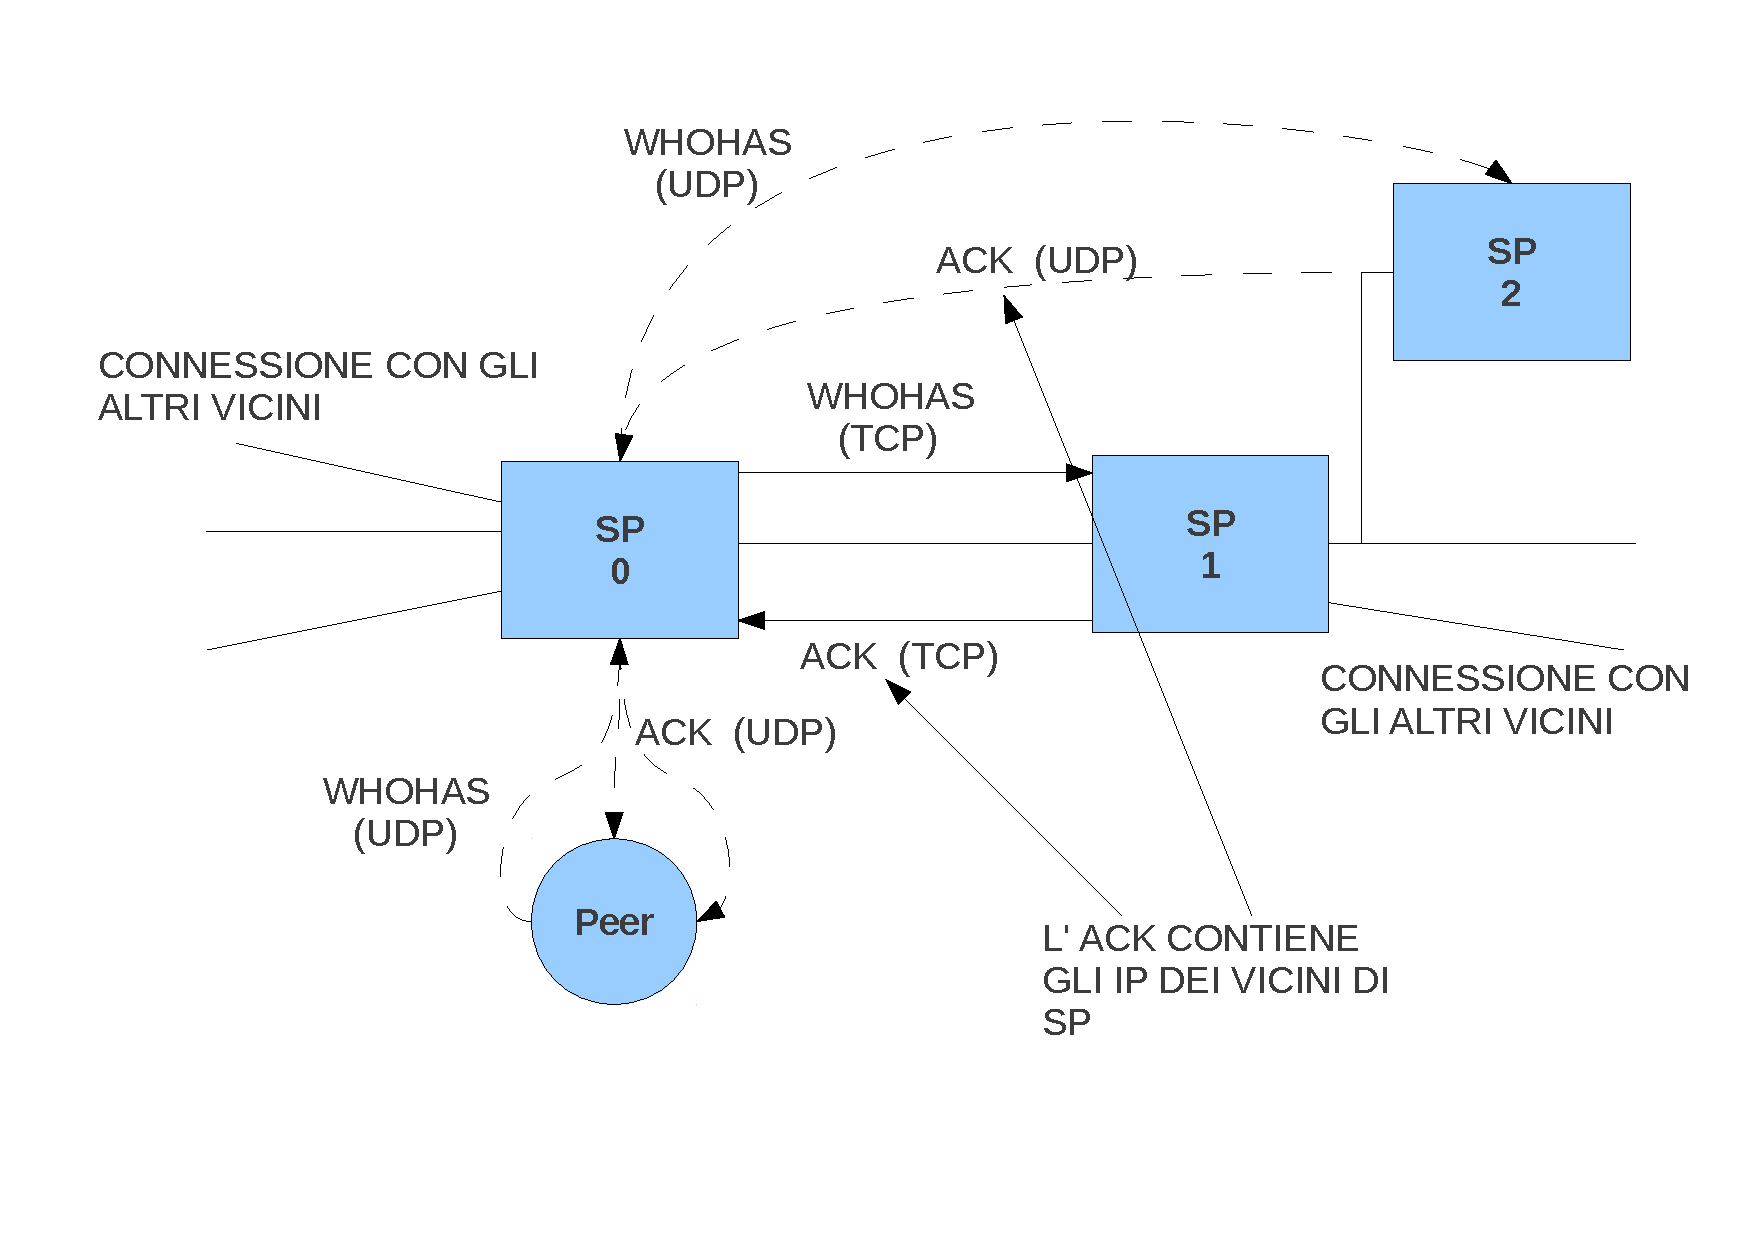
\includegraphics[width=12cm]{img/whhs_sull_overlay}}
\caption{Propagazione della whohas sull'overlay\label{whhs_overlay}}
\end{figure}



Come si può vedere un superpeer che riceve la whohas dal suo peer la inoltra ai suoi vicini in TCP, in figura si è evidenziato lo scambio con uno solo di questi il quale quando inoltra l'ack, comunica anche gli indirizzi IP dei superpeer adiacenti (sempre utilizzando TCP), ai quali verrà successivamente inoltrata la whohas questa volta però in UDP.\linebreak
I superpeer, che hanno ricevuto la whohas, a loro volta inoltreranno l'ack in modo simile ai vicini con la sola differenza di utilizzare UDP come protocollo di trasporto, e la ricerca proseguirà nel modo descritto fino a quando non si verificheranno determinate condizioni discusse successivamente.     

\subsubsection{Fine ricerca}
Il controllo sulla fine della ricerca è implementato allo scopo di non congestionare la rete di overlay, in quanto senza questo controllo i pacchetti di whohas e di ack circolerebbero all'infinito nella rete. Nel metodo implementato, il superpeer che origina la query contatta iterativamente alcuni superpeer della rete, finché non si verifichi almeno una delle seguenti condizioni:\linebreak
\begin{itemize}
\item Il superpeer che ha originato la query ha contattato un numero massimo di superpeer(configurabile tramite file config);
\item Il superpeer che ha originato la query ha ottenuto in risposta un numero massimo di peer che contengono il file cercato (configurabile tramite file config);
\item Il peer che ha effettuato la whohas al superpeer decide di fermare la ricerca(Stop UDP). 
\end{itemize}

\textbf{STOP\_UDP} \linebreak
La stop\_UDP viene richiamata dal peer quando l'utente sceglie il comando di STOP durante una ricerca, dopo di chè il peer invierà un messaggio di STOP in UDP con un meccanismo di ritrasmissione come tutti gli altri messaggi UDP. Quando il superpeer riceve il messaggio di STOP della ricerca dal peer cancellerà dalla sua lista di query la query corrispondente al peer(che riconosce nella lista tramite l'indirizzo IP da cui gli arriva il messaggio di STOP), in questo modo anche se gli dovessero arrivare altre risposte alla query appena cancellata(se quando gli arriva lo STOP aveva già inoltrato qualche whohas di cui attende risposta), cercando nella lista delle query pendenti l'id e non trovandolo 
scarterà il pacchetto evitando così di ritrasmetterlo ad altri superpeer, ed inoltre non invierà le risposte ricevute neanche al peer in quanto per lui ormai la ricerca si è conclusa.\linebreak